\documentclass{article}
\usepackage[utf8]{inputenc}
\usepackage[acronym]{glossaries}
\usepackage{biblatex}
\usepackage[colorinlistoftodos]{todonotes}
\usepackage{graphicx}
\usepackage{pgfplots}
\usepackage{fancyvrb}

\addbibresource{bibliography.bib}


\title{Detekt-hint -- Detection of programming principle violations}
\author{Marius Kohmann}
\date{June 2020}


\newacronym{ast}{AST}{Abstract Syntax Tree}
\newacronym{solid}{SOLID}{\textbf{S}ingle responsibility, \textbf{O}pen–closed, \textbf{L}iskov substitution, \textbf{I}nterface segregation, \textbf{D}ependency inversion}
\newacronym{dry}{DRY}{Don't Repeat Yourself}
\newacronym{srp}{SRP}{Single Responsibility Principle}
\newacronym{ocp}{OCP}{Open-Closed Principle}
\newacronym{lsp}{LSP}{Liskov Substitution Principle}
\newacronym{isp}{ISP}{Interface Segregation Principle}
\newacronym{dip}{DIP}{Dependency Inversion Principle}
\newacronym{lcom}{LCOM}{Lack of Cohesion Of Methods}
\newacronym{pr}{PR}{Pull Request}
\newacronym{ntnu}{NTNU}{Norwegian University of Science and Technology}

\begin{document}

\maketitle

\begin{abstract}
	%Sample IMRaD abstract: 
	
	
	
\end{abstract}


\clearpage
\tableofcontents
\clearpage
\section{Introduction}
Writing maintainable and high quality code is an important part of software engineering. Various people define software maintainability differently, but a commonly
accepted collection of quality attributes include extensibility, modularity, testability and understandability. To help developers write code with those attributes, well defined rules and conventions have been developed. They are often enforced by the use of tools commonly referred to as linters. Design principles is another invention that has been created to help developers write code that adheres to the aforementioned quality attributes. Unfortunately, many of the principles are not formal and is often open for interpretation and subject for debate. Therefore, correct appliance of the principles often requires reasoning about the business domain and predicting future changes to the code base. The absence of correctly applied design principles triggers maintainability problems and is often a breeding ground for bugs, refactoring\footnote{From Wikipedia: Process of restructuring existing code without changing its external behavior \cite{refactoring}.} tasks and technical debt\footnote{From Wikipedia: Concept in software development that reflects the implied cost of additional rework caused by choosing an easy (limited) solution now instead of using a better approach that would take longer \cite{technicalDebt}.}. Consequences include increased development time, inaccurate estimations causing lost deadlines and higher costs of introducing new developers to the project.

%Objective
The objective of this study is to develop knowledge about detecting violations of programming principles using the design science methodology. The design science methodology involves development of an innovative product through short iterations that includes the use of prototypes and continuous feedback. The study will present the inner workings of the product as well as a detailed evaluation of the final artifact.

The outline of the paper is as follows; Section \ref{background} gives some background information and an introduction to the topics of writing code with high quality and code analysis. Section \ref{methodology} describes the methodology of the research process. Section \ref{relatedwork} gives some insight in related work in the area and section \ref{results} presents the developed artifact, and a detailed evaluation of it. Section \ref{discussion} discusses the results, and lastly in section \ref{conclusion} we conclude the paper.  

\section{Background}
\label{background}
To be able to develop a tool for detection of programming principle violations using the design science methodology there are a handful of \todo{better word} subjects you need to be familiar with. The following sections will give a brief introduction to them.


\subsection{Code analysis}
\todo{rewrite this to fit programming principles and PSI}
To help developers of software systems adhere to these concepts and conventions tools for code analysis have been developed. In code analysis we differentiate between two types of code analysis, dynamic code analysis and static code analysis. \textit{Dynamic code analysis} is done by analysing programs being executed on a processor, while \textit{static code analysis} is purely based on analysis of the source code. Since dynamic analysis is based on program execution it has the advantage of being able to measure the actual CPU, memory and energy performance of the application. 

%It can also gather information about the system that would be hard to detect using static code analysis. Examples include discovery of dynamic dependencies using reflection, or actual application usage. However, that does not mean that static code analysis is not able to target performance or dynamic aspects of source code.

As we search to improve the source code, we have chosen to focus on static code analysis. The static analysis is done by parsing the source code, creating an \gls{ast} and then analyzing the tree for violations of the aforementioned concepts and conventions. Figure \ref{fig:ast} shows a simple example \gls{ast} where a static analysis tools could detect that the expression \texttt{x == 1} always evaluates to \texttt{true} and that the variable \texttt{y} is never used. The tool could then suggest that the branching is unnecessary and that the \texttt{y} variable is removed.  

\todo{Exchange this for an example with useCompositionInsteadOfInheritance rule}
\begin{figure}[h!]
	\centering
	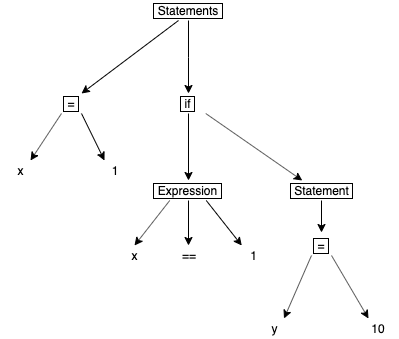
\includegraphics[width=\linewidth/2]{report/ast.png}
	\caption{Simple \gls{ast} of x=1; if (x == 1) \{y = 10;\}}
	\label{fig:ast}
\end{figure}


\subsection{Design science}
Design science is a research methodology that focuses on getting knowledge through development of innovative artifacts. The methodology provides specific guidelines for evaluation and iteration in research projects.
\todo{insert image of design science methodology}

\subsection{Prototyping}

horizontal and vertical prototypes. high and low res prototypes.

\subsection{Design principles}
Design principles (also called programming principles) are a set of guidelines that programmers should follow to avoid bad design. According to Robert C. Martin \cite{robertcmartinprinciples} there are three characteristics of bad design that the design principles will help reduce:

\begin{enumerate}
	\item Rigidity - It is hard to change because every change affects too many other parts of the system.
	\item Fragility - When you make a change, unexpected parts of the system break.
	\item Immobility - It is hard to reuse in another application because it cannot be disentangled from the current application.
\end{enumerate}

A common set of design principles that often is referred to is the \gls{solid} principles and \gls{dry} principle. The design principles are often abstract and verification requires knowledge and reasoning about the business domain. They are therefore hard to verify using code analysis. 

\todo{In depth description of SOLID principles as they are important in the tool}


One could easily think that \gls{dry} could be verified through looking at similar code, but it turns out that it is not that simple. Two code snippets could be exact copies of each other, but still not violating \gls{dry} if the two snippets would change for different reasons. 

This is the core problem i am facing in this study - helping the developers with these decisions even if the problem could not be verified.


\subsection{False positives}
As stated above, design principles are hard to verify and is the reason why very few tools cover them. Because we could not be 100\% sure if a design principle is followed we would end up with our tool reporting issues, that in reality are not issues. We call these \textit{false-positives}. These create noise and are obtrusive for the developer, so it is important to keep the false-positive rate as low as possible.


\subsection{MVP}

\section{Related work}
\label{relatedwork}
Ndepend. Jarchitect. 

\section{Methodology}
\label{methodology}
This study will follow the Design Science methodology which is presented in (A Design Science Research Methodology for Information Systems Research) \cite{10.2753/MIS0742-1222240302}. It is selected because it fits the process of building a innovative software artifact. The software artifact will be created through a series of iterations that include the follow activities; problem identification/understanding and motivation, definition of objectives for a solution, design and development, demonstration/testing, evaluation, communication.  An illustration of the design science methodology can be seen in figure \ref{fig:designScience}. As can be seen in the figure is important to notice that the activities is not done in any particular order, but in that order as seen required.  \todo{Should i create my own figure that includes problem understanding? Or is this not part of design science? I would then argue that i slight modification of the method should be used that includes iterations on the first step.}. I will elaborate on how the different activities is applied to the project below. 

\subsection{Problem identification}
The problem is that important design decisions are'nt considered before it is too late, so that bad design end up in production code, creating maintainability problems.


The problem is that very few tools for detecting design principle violations exists. As mentioned in \ref{relatedwork}, the existing tools analyze the whole codebase and is not integrated with the development process. Using the existing tools can be good for project level analysis activities, and finding areas of improvement. The tools also lack support for many import design principles.


What Detekt-hint is looking to improve is the tight integration with the development process and helping the developer taking good decisions while the developer is in the context.


\hfill \newline
These two goals can be summarized as two research questions:
\hfill \newline
\hfill \newline
\textbf{RQ1}: How can violations of design principles be identified? \newline
\textbf{RQ2}: Can we accept a higher rate of false-positives? \newline
Is the value of a true-positive worth more than the sum of all the false-positives? It all boils down to time=money. Time to overlook times the amount of false-positives vs time that was saved because an important design decision was made as a result of the true-positive identification.


% Motivation - justyfing the value of a solution
Get some sources that design principles are important and would cost much less to fix now than later. Also some sources on developer context-change that is beneficial.


before the code is merged into 


can be used to find where to start reducing technical debt, but is not highly integrated into the development process and asks the questions if the newly developed code is good - while the developer is in the context. The developer can do a consoucious decision to do refactoring before the code is merged in. 

Current tools (linters) have low false-positive rate, but are not able to target important things like the architecture of the application. This tool will be able to target the architecture, but with higher false-positive rate, and through the format of QA hopefully not disturbing the development process too much. 


The motivation is that programming principles are important because they create structure and lay the foundations of building and extending the product.

based on the pre study and own needs i decided to build the tool.

Ok to reference popularity on github/reddit, but can be misvisende and it is important to not take the response there for god fisk.

\subsection{Define objectives of a solution}
Involves creating a specification of the solution.

\subsection{Design and development}
Involves the development of the final software artifact and both horizontal and vertical prototypes. Prototypes is used early in the development phases to quickly be able to evaluate the product. Horizontal prototypes should be created to early demonstrate a broad view of the final artifact. Vertical prototypes will be used to elaborate on technical challenges and the workings of specific features. 
 
\subsection{Demonstration}
Gather people for an workshop and presentation of horizontal prototypes. Important to create a structured schema with questions and impressions to get feedback in a structured way that can be used to evaluate the different features.
 
\subsection{Evaluation}
I find that it is super hard to get feedback on something. I think more rules needs to be implemented to be able to get some valueable feedback. Un-structured feedback trough Reddit. Evaluation of github bot as platform for feedback. Evaluation of implemented rules. Evaluate how often the rule gets triggered using a built software system / vs the noise it creates. Evaluate impact on decisions - e.g a commit introduced some inheritance, and later it was found out that inheritance caused trouble. Simulation on other projects to find bugs and false-positives. Used it to further improve the rules and reduce the noise.

Gather a group of Kotlin/Android entusiasts for a workshop where one could order pizza and code using this tool. Focus on feedback. Could for example analyze some code that they know and give some feedback on whether it is useful or not. What would have been useful?

Not that much focus on creating and hitting bullseye with the product, more about the feedback itself and how to respond to it.

Multiple evaluation methods used on different stages of the project: Evaluation running the program on others code, evaluation using a workshop with focus on feedback and usage, evaluation of the initial project using reddit etc.

However, i posted an image of the MVP on Reddit/Kotlin, and it quickly got so many upvotes that it was top this week in under 12 hours. 

\subsection{Communication}


My needs for this solution. Needs a AST to analysis and a framework to help me with this. Need a way of creating a report of the analysis and feed it to something else that can post on github. 


\section{Results}
\subsection{Prototypes}
\subsubsection{Horizontal prototype}
The horizontal prototype was built by creating sample \gls{pr} in a sample repository on Github\cite{sample-repository}, and then commenting on the \gls{pr}'s with the bot user. An example from the prototype is presented in figure \ref{fig:liskov}. 

\begin{figure}[h!]
    \centering
    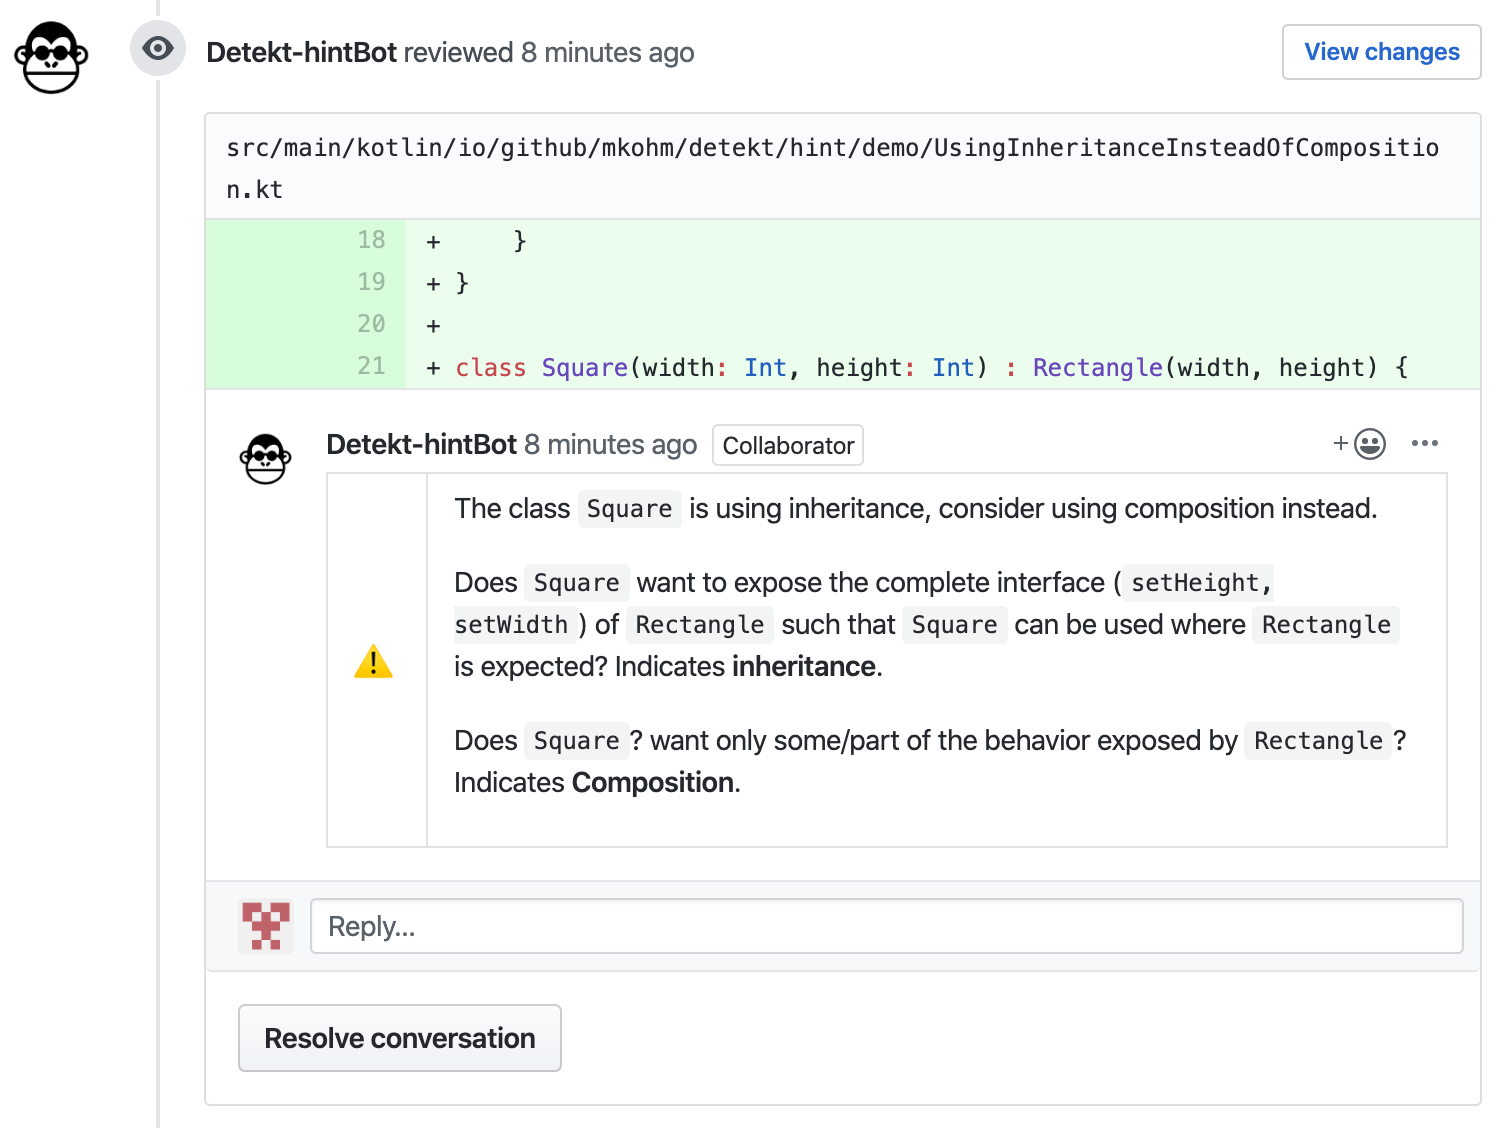
\includegraphics[width=\textwidth]{../demo.png}
    \caption{Prototype of the composition over inheritance / \gls{lsp} rule}
    \label{fig:liskov}
\end{figure}

% What did i find when using this prototype? What changes does the product need, or does it confirm that i am on the right path?

The schema used for evaluation of the prototype, the participants answers and selected images of the prototype can be found in appendix \ref{horizontal-prototype}. The full prototype can be found in the sample repository \cite{sample-repository}. 

\subsubsection{Vertical prototype}
To get structured feedback on the prototype it 
Horizontal prototypes with github PR samples with bot commented. Was easily created by pushing code to repo and logging in as the bot. Should create samples that demonstrates possible false positives as well as true positives. 

\subsection{Workshop}
Schema:
Who is the participants, some background information on them. What did the participants say. What is the takeaway from the workshop? What did i change in the product after having the workshop?

What is the goal, how should i reach the goal of the workshop. Keep the workshop structured.

\subsection{}

\subsection{Short recap of the development process}
Creating a vertical prototype with a simple rule (usecomposition rule) to see if this project it technically possible within the time frame of a masters thesis. 

The schema for the workshop can be found in appendix \ref{workshop-schema}.


\subsection{Detekt-hint specification}
Specification of all the rules.

\subsection{Architecture}
A diagram of how everything interacts with each other.

\subsubsection{Detekt}
Detekt is a static analysis tool for kotlin. Which provides access to a framework for rule creating for analyzing code and reporting warnings.

Detekt gives us access to IntelliJ PSI for analyzing Kotlin code. The PSI is built on top of the \gls{ast} provided by the kotlin compiler, and provides utility methods for modifying and querying of the underlying \gls{ast}.

Type resolution?

\subsubsection{Detekt-hint}

\subsubsection{Danger}

\subsubsection{Danger detekt plugin}

\section{Discussion}
\label{discussion}

\section{Future work}
Implement more rules.
Reducing the amount of false positives.

Providing more context and/or possible solutions in the comments. Images or graphs explaining.
Increasing the performance.
Easing the setup process. Github app? Direct integration with the repository with no setup. A tool like code-climate that does not need any configuration. Plus of tool like this: all setup is in source control. Downside: could be tedious to set up or not all team members want to use it.

\section{Conclusion}
\label{conclusion}

\section{Acknowledgements}
\label{acknowledgements}
Thanks to supervisor, all participants in workshop and prototype sessions.

\printbibliography

\appendix
\label{appendix}
\clearpage
\chapter{Appendix}

\section{Horizontal prototype}
\label{horizontal-prototype-images}

\begin{figure}[h!]
    \centering
    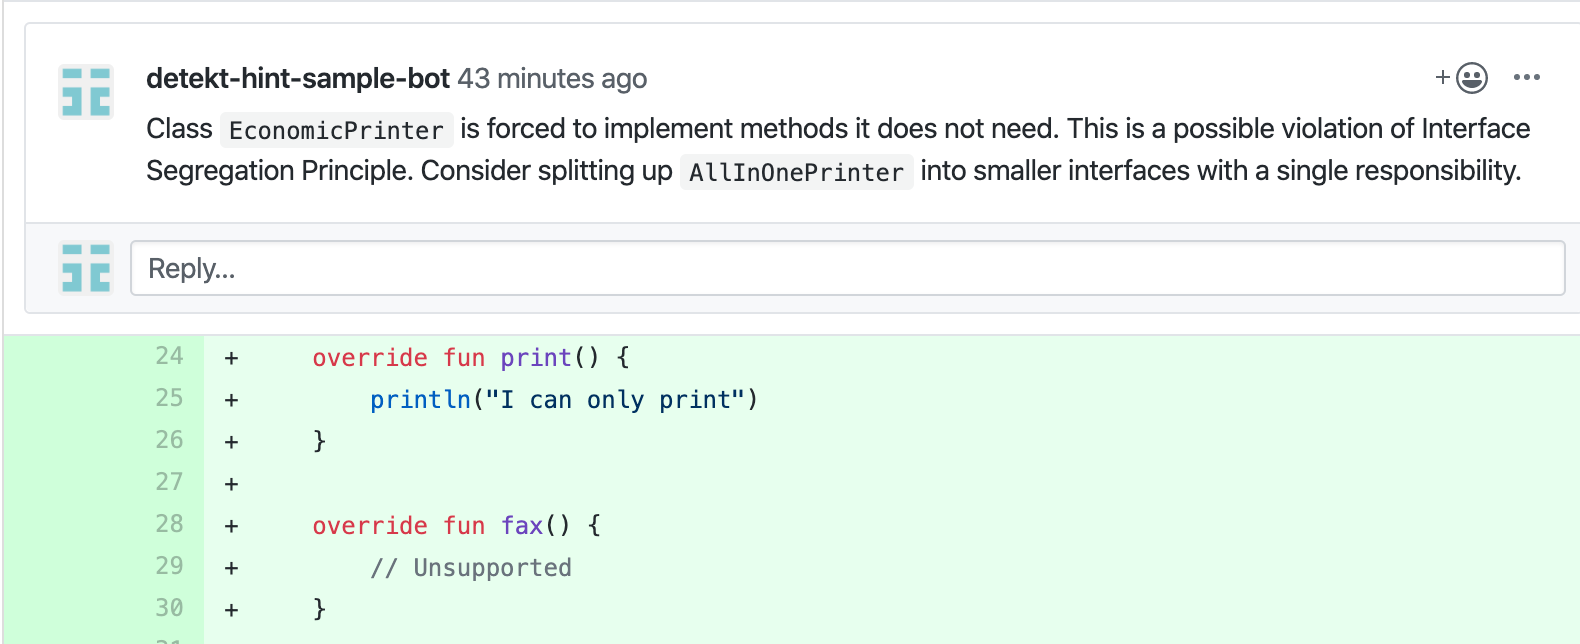
\includegraphics[width=\textwidth]{../images/comment_isp.png}
    \caption{Screenshot of the horizontal prototype showing the \gls{isp} rule. It has detected an empty method, which is a sign of violating the \gls{isp}. In this case the \texttt{EconomicPrinter} implements methods from \texttt{AllInOnePrinter} which it does not need. A solution would be to define separate interfaces for each of the responsibilities (e.g \texttt{Printable, Faxable, Scanable}) and let the concrete implementations of printers implement the interfaces they need.}
    \label{fig:isp}
\end{figure}


\begin{figure}[h!]
    \centering
    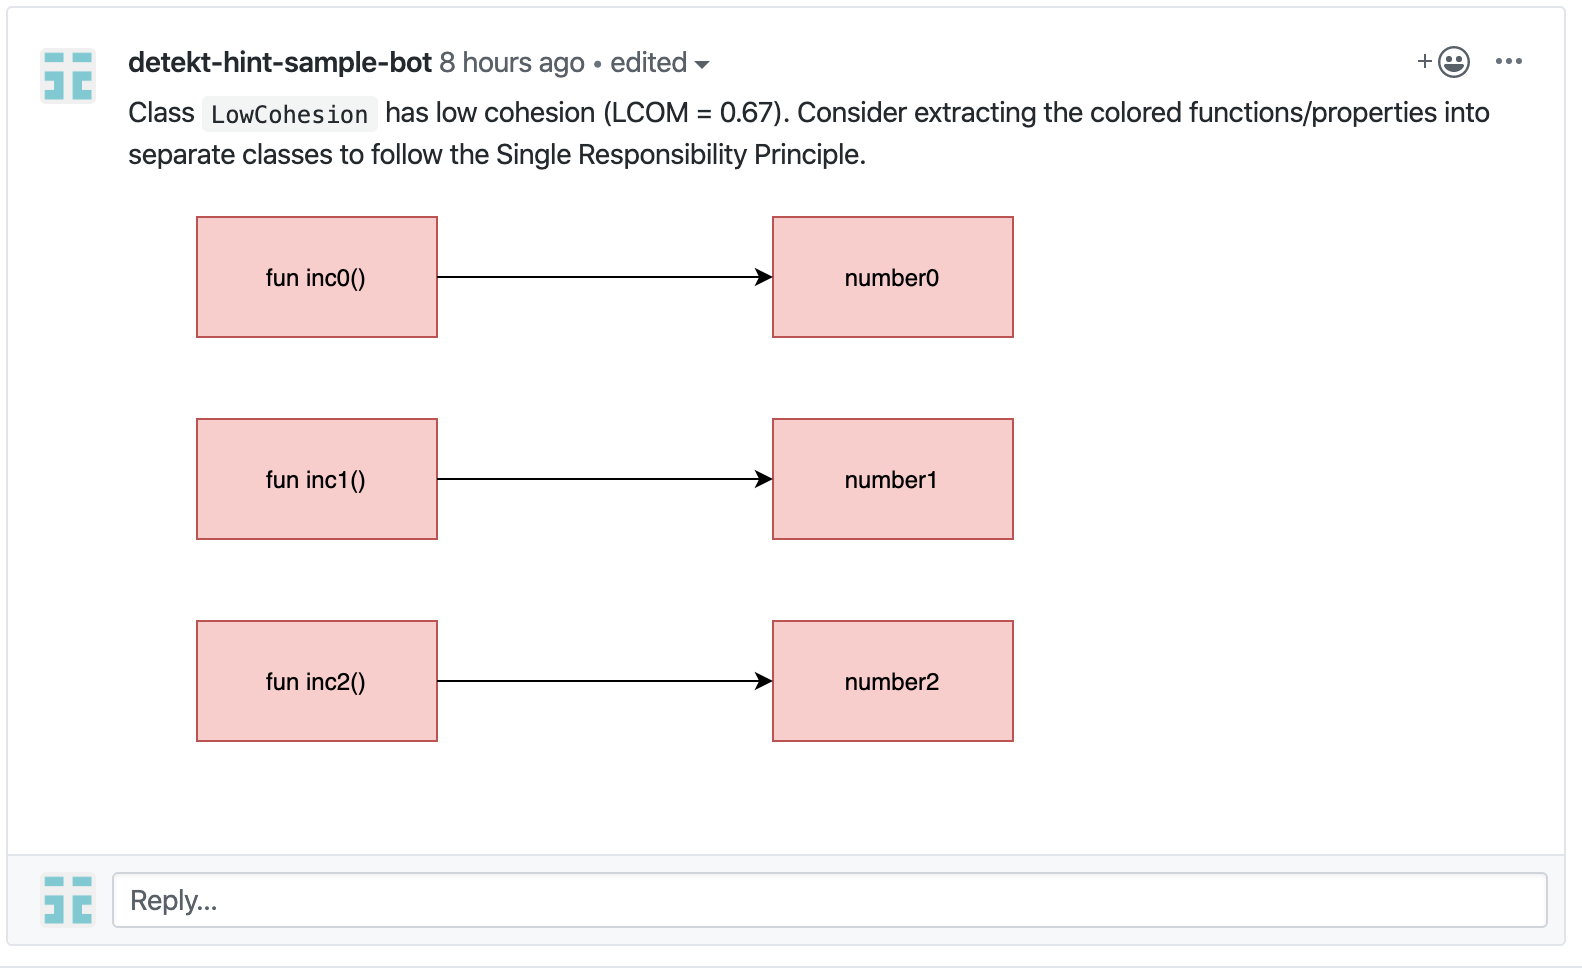
\includegraphics[width=\textwidth]{../images/comment_lackOfCohesion.png}
    \caption{Screenshot of the horizontal prototype showing the \gls{lcom} rule, with a visual representation of the lack of cohesion. The figure shows which fields that are referenced from each of the methods in the class. In this case all the methods of the class references their own separate field. This indicates that each of the methods and corresponding fields have separate responsibilities within the class. This would therefore be an indication of violating the \gls{srp}.}
    \label{fig:lcom}
\end{figure}


\begin{figure}[h!]
    \centering
    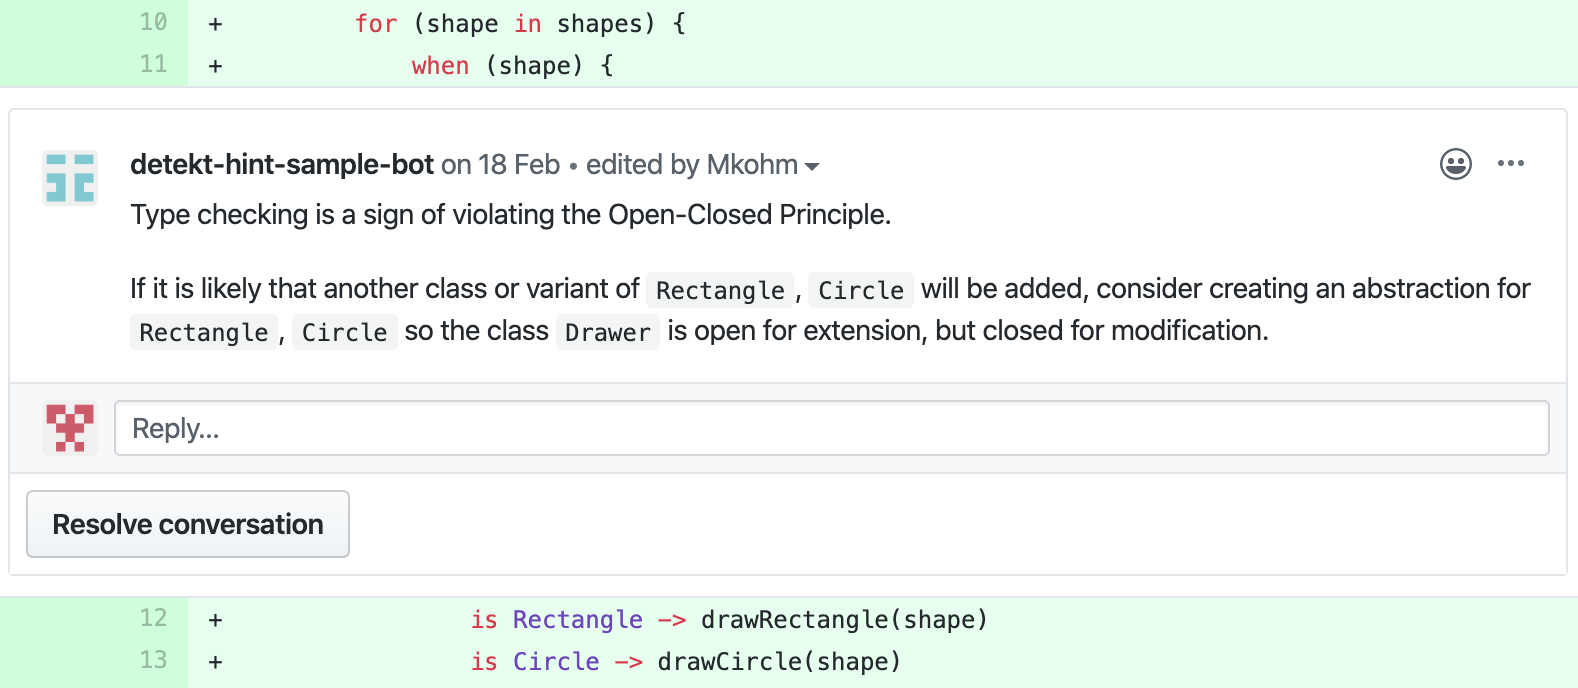
\includegraphics[width=\textwidth]{images/comment_ocp2.png}
    \caption{Screenshot of the horizontal prototype that shows the \gls{ocp} rule, using a simple program for drawing shapes. In this case the rule detected checking of concrete implementations to control flow. The rule suggests creating an abstraction for \texttt{Rectangle}, \texttt{Circle} (e.g an interface \texttt{Shape} with a \texttt{draw} method that all \texttt{Rectangle} and \texttt{Cirle} should implement) such that eventual new shapes added to the program would not need to modify existing code. }
    \label{fig:ocp}
\end{figure}


\begin{figure}[h!]
    \centering
    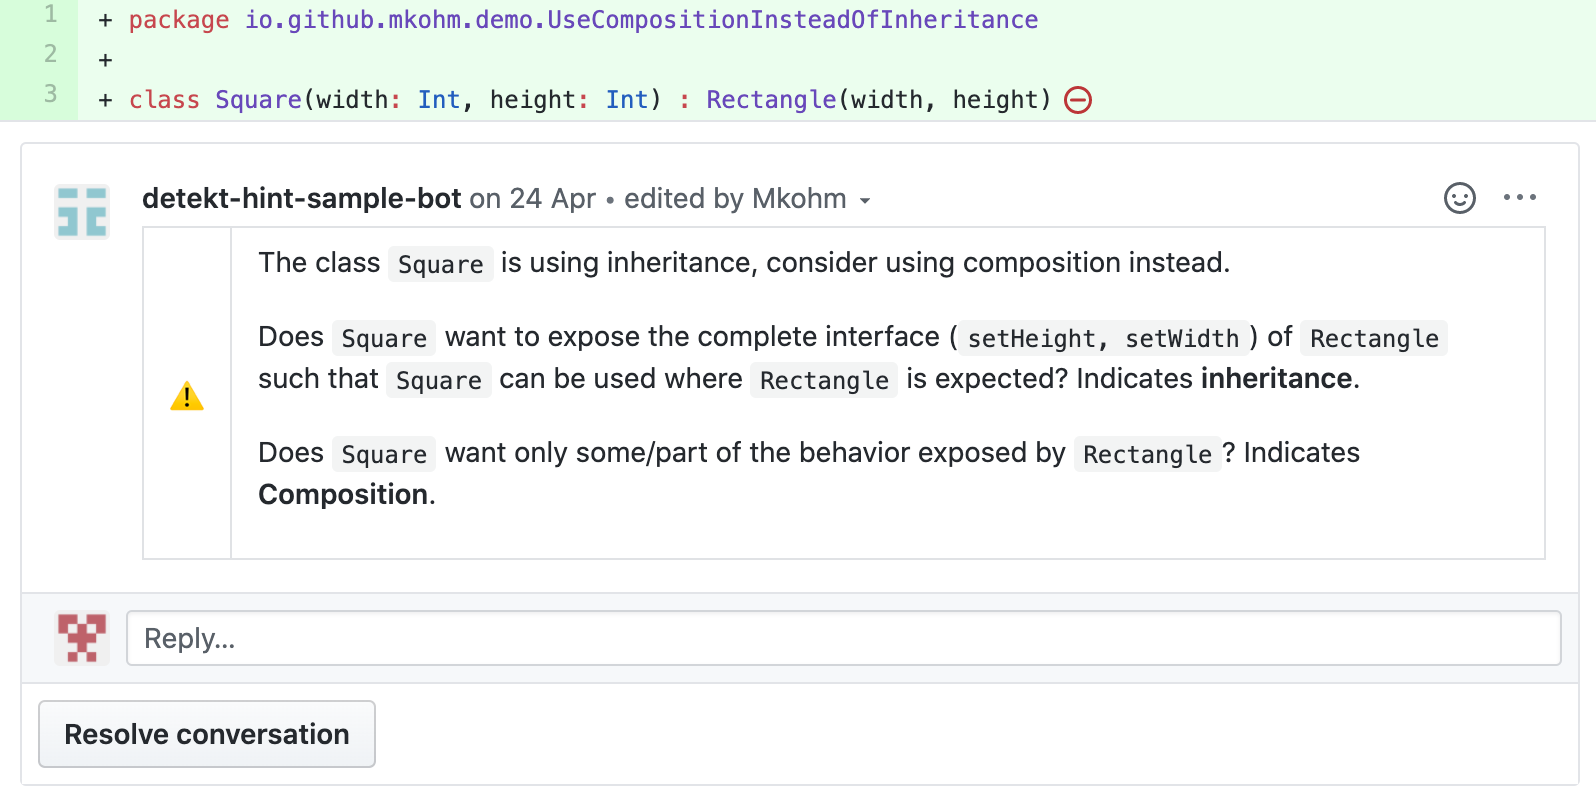
\includegraphics[width=\textwidth]{images/horizontal-prototype-coh.png}
    \caption{Screenshot of the horizontal prototype that shows the \gls{coi} rule. The rule suggests the use of composition instead of inheritance, and helps testing if the classes adheres to the \gls{lsp}. In this case, the classical Square - Rectangle problem is presented. \texttt{Square} should not be derived from \texttt{Rectangle} as it would violate the \gls{lsp}. \texttt{Square} does not functionally behave like \texttt{Rectangle} as squares by definition have the same width and height. \texttt{Rectangle} should have two independent methods for changing its size, but clearly these methods is not appropriate for the \texttt{Square}. }
    \label{fig:liskov}
\end{figure}

\clearpage

\section{Semi-structured interview schema}
\label{semi-structured-interview-schema}
\subsubsection*{Participant number:} What is the number of the participant.
\subsubsection*{Background:} What is the participants background. Experience with software architecture? Knows and uses design principles? Experience with Kotlin?
\subsubsection*{Presentation of rules - For each rule}
\begin{enumerate}
    \item Present the rule. 
    \item Make sure the participant understands the importance of the rule.
    \item When will the rule give a warning?
    \item When will the rule incorrectly give a warning? Will it report false-positives too often? Suggestions on how to reduce the amount?
    \item How much context is needed? Shorter or longer comments? Should include suggestions on possible solutions? Is the comment understandable? Something missing?
\end{enumerate}

\subsubsection*{Other} 
- When reviewing code, what do you think is tedious, and could it be automated?
- Are there any rules/principles missing?

\clearpage
\section{Semi-structured interview results}
\label{horizontal-prototype-interview-results}

\textbf{Participant number:} 1 \newline
\textbf{Background:} Studies computer science at \gls{ntnu} with a specialization in computers and systems software. Has experience with developing apps for iOS and web and back-end development. Interested in Software Architecture and writing software of high quality. \\
\textbf{Experience with design principles:} Some \\\\

\noindent \gls{coi}: Could be useful, but potentially have too many false positives. For testing the participant often creates Mock objects that inherits from the class he wants to Mock, and then overrides methods. The participant think there is too few cases where this rule will be useful. Suggestions: Reduce the amount of positives by disabling checks for classes with names; Mock. User could specify which class names or a pattern to ignore. Should revisit sentence number two about composition, it could be misleading.\\\\

\noindent LCOM1: Very useful because calculating such a value is'nt something you do while coding. Positive that you can change the threshold of the rule. Suggestion: Which fields and methods could i extract? A comment that suggests a solution. \\\\

\noindent LCOM2 (With refactoring visualization): Look more at further analysis to find out what can be extracted. Look into dependencies between function calls as well. Diagram looks cool, but does not give any more value than some plain text explaining what can be extracted. \\\\

\noindent \gls{ocp}: Somewhat useful. Should have a more specific comment saying if you are doing enum switching or instanceOf checking. \\\\

\noindent \gls{isp}: Could be useful. Suggestion to count number of usages of calls in the interface to see which method calls that is not used by any of the classes that implement the interface. \\\\

\noindent Other: Tools for detecting complicated expressions that can be extracted out as a separate method with a descriptive name. Blocks of code should be extracted out as separate methods so that lines of code that belongs together has its own scope. 
\clearpage


% Netlight
\noindent\textbf{Participant number:} 2 \newline
\textbf{Background:} Works as a software developer for Netlight, 2 years of professional developer experience. Experienced with Kotlin development and with architecture and design of software systems.\\
\textbf{Experience with design principles:} Yes \\\\

\noindent \gls{coi}: Positive about the rule, but is concerned about not showing warnings when deriving from third party libraries. This is a case where one also should think about using composition instead of inheritance. Suggests to remove this logic, and instead provide configuration options for packages that should not be reported as violations when derived from.  \\\\

\noindent \gls{lcom}: Nothing special. \\\\

\noindent \gls{ocp}: Useful for both instance of checking and enum switching. Enums in Kotlin are powerful, so switching on them is in many cases not needed and polymorphism is used instead.\\\\

\noindent \gls{isp}: Could be useful. May need to handle TODO's specially. \\\\

\noindent Other: In general positive to the tool, and think it has potential. Good that it is easy to ignore warnings, with just a click. It needs more rules before considering using it. For example including detection of Java anti-patterns and ensuring that Kotlin code is idiomatic. For example static methods and places where data-classes could be used. The tool could be used as "training wheels" in a team, where one gradually could disable more rules to not create unnecessary noise in the development.

\clearpage
\section{Final prototype}
\label{final-artifact}
\begin{figure}[h!]
    \centering
    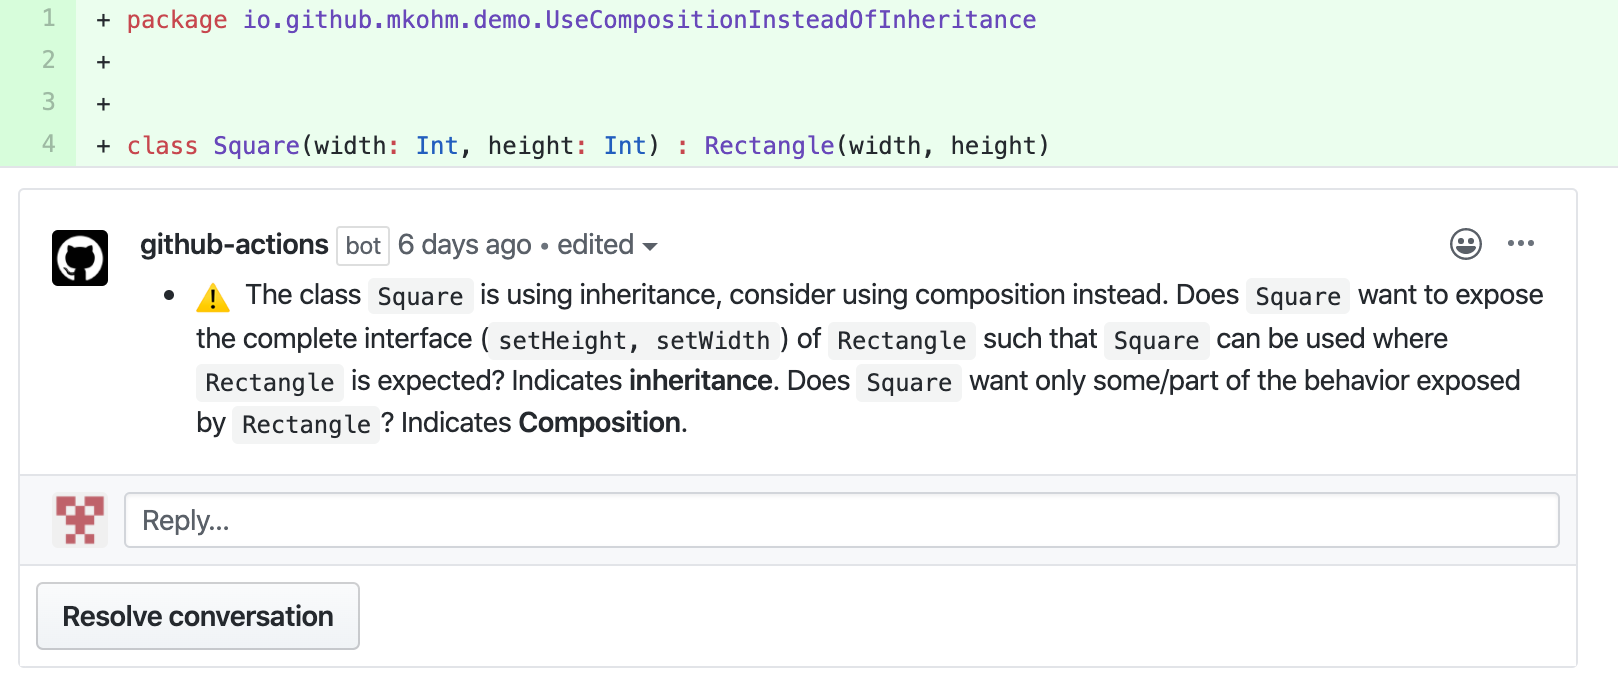
\includegraphics[width=\textwidth]{images/final_coh.png}
    \caption{Screenshot of the final prototype that shows the \gls{coi} rule. The rule suggests the use of composition instead of inheritance, and helps testing if the classes adheres to the \gls{lsp}. In this case, the classical Square - Rectangle problem is presented. \texttt{Square} should not be derived from \texttt{Rectangle} as it would violate the \gls{lsp}. \texttt{Square} does not functionally behave like \texttt{Rectangle} as squares by definition have the same width and height. \texttt{Rectangle} should have two independent methods for changing its size, but clearly these methods is not appropriate for the \texttt{Square}.}
\end{figure}

\begin{figure}[h!]
    \centering
    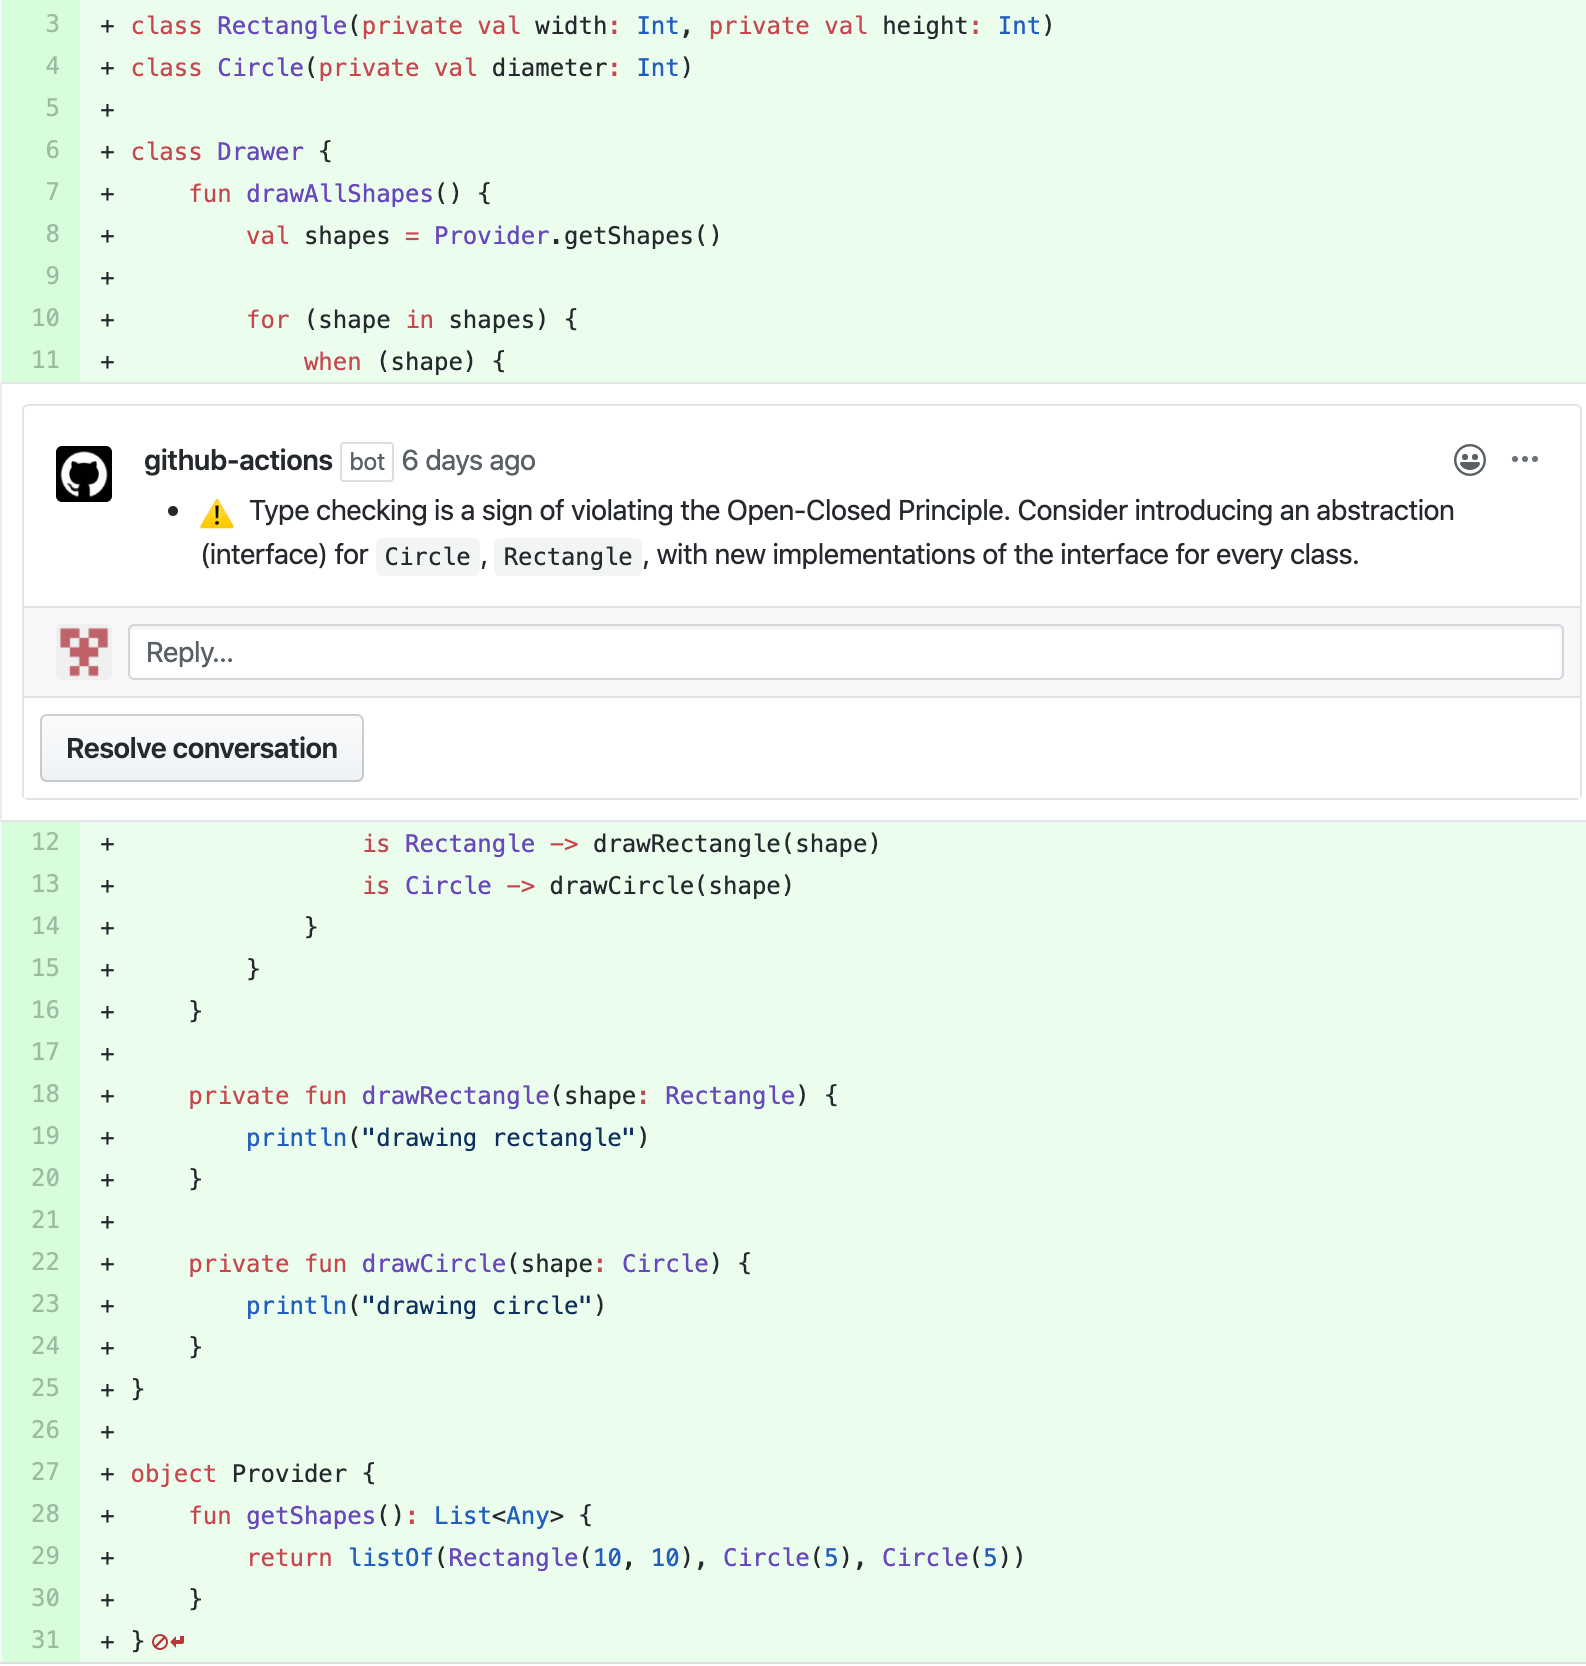
\includegraphics[width=\textwidth]{images/final_ocp.png}
    \caption{Screenshot of the final prototype that shows the \gls{ocp} rule, using a simple program for drawing shapes. In this case the rule detected checking of concrete implementations to control flow. The rule suggests creating an abstraction for \texttt{Rectangle}, \texttt{Circle} (e.g an interface \texttt{Shape} with a \texttt{draw} method that all \texttt{Rectangle} and \texttt{Cirle} should implement) such that eventual new shapes added to the program would not need to modify existing code.}
\end{figure}

\begin{figure}[h!]
    \centering
    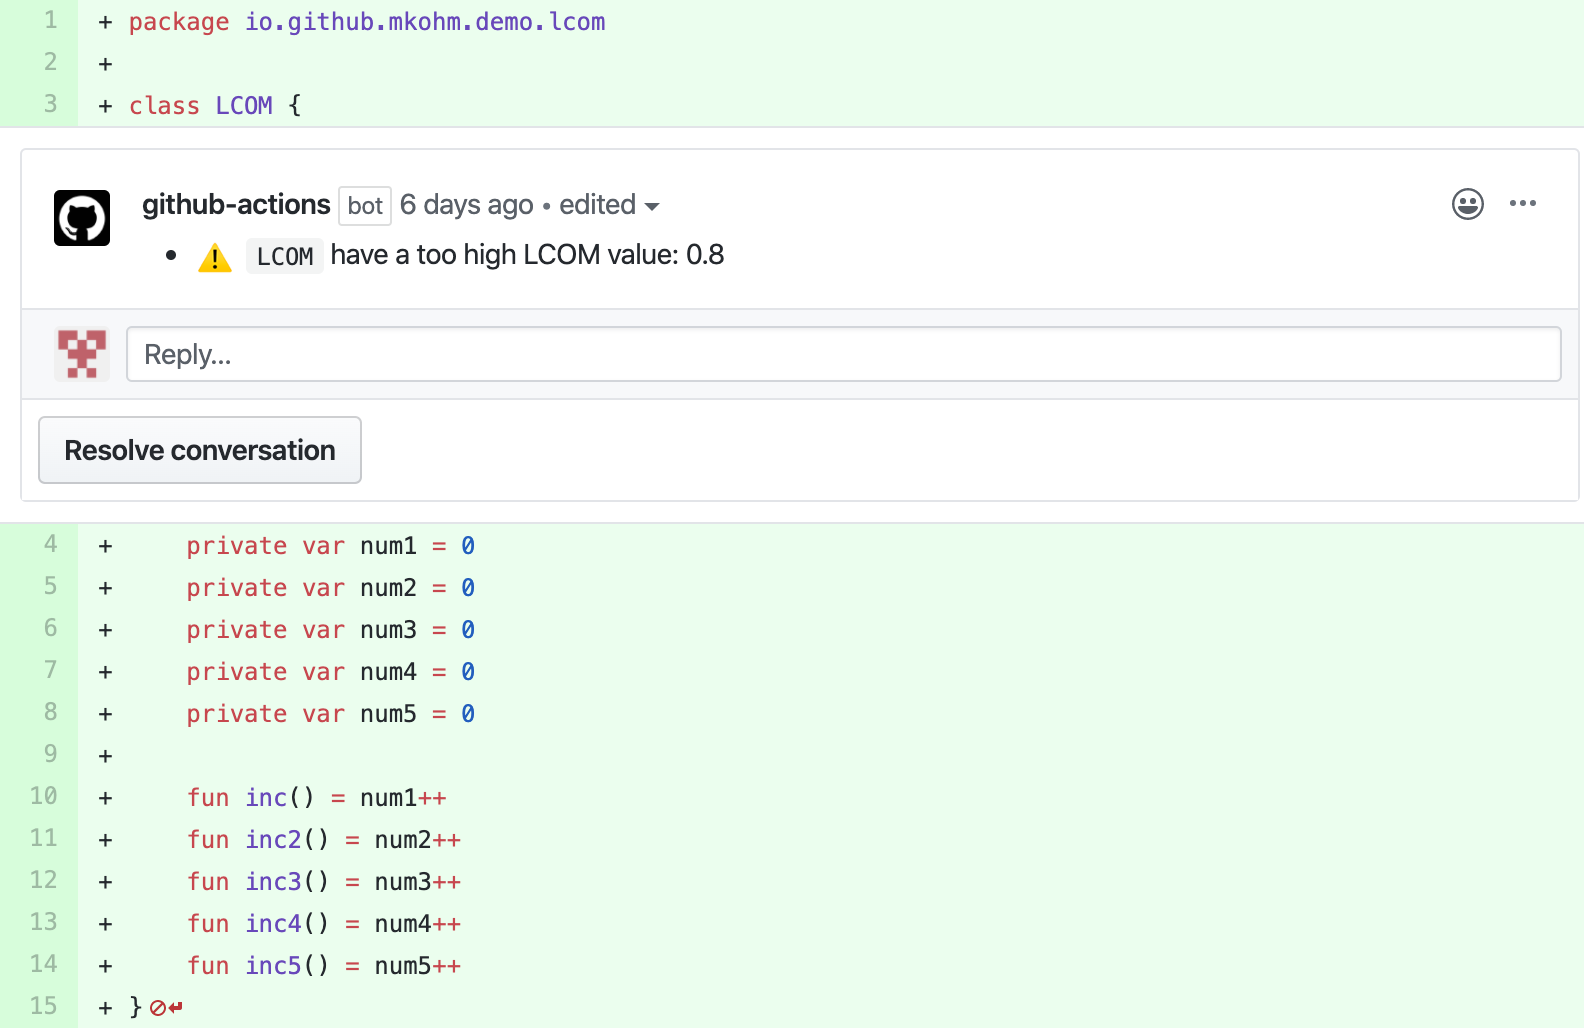
\includegraphics[width=\textwidth]{images/final_lcom.png}
    \caption{Screenshot of the final prototype showing the \gls{lcom} rule. This is an indication of violating the \gls{srp}, due to low cohesion in the class. In this case, each of the methods reference their own field, telling us that there is no relationship between the different methods, and that they don't need to exist in the same class.}
\end{figure}

\begin{figure}[h!]
    \centering
    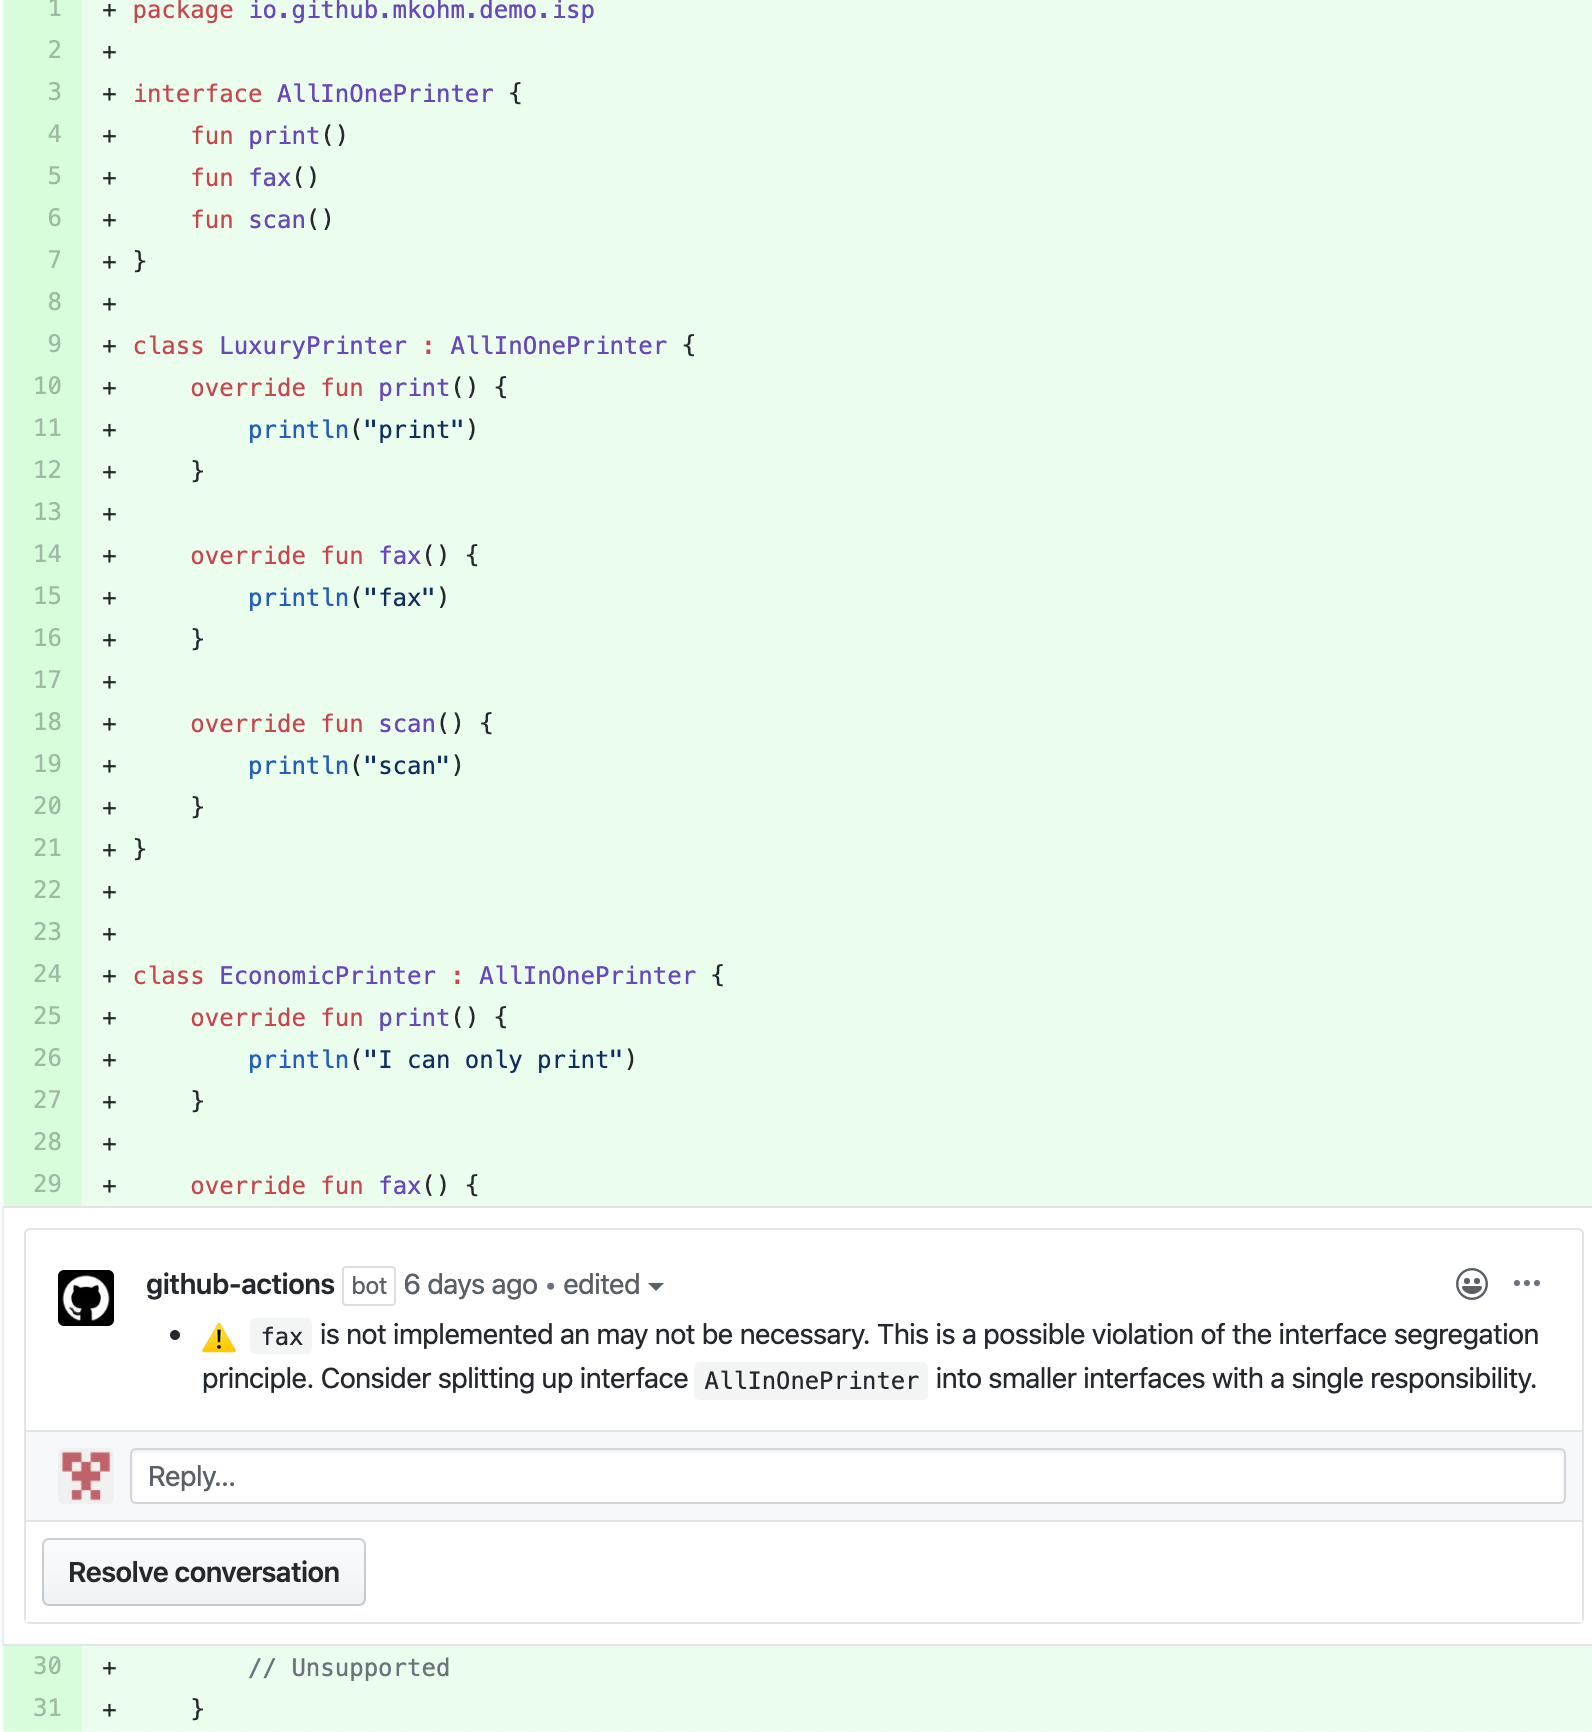
\includegraphics[width=\textwidth]{images/final_isp.png}
    \caption{Screenshot of the final prototype showing the \gls{isp} rule. It has detected an empty method, which is a sign of violating the \gls{isp}. In this case the \texttt{EconomicPrinter} implements methods from \texttt{AllInOnePrinter} which it does not need. A solution would be to define separate interfaces for each of the responsibilities (e.g \texttt{Printable, Faxable, Scanable}) and let the concrete implementations of printers implement the interfaces they need.}
\end{figure}

\end{document}